Il termine \textbf{``sicurezza"} si riferisce alle tecniche, ai processi e ai provvedimenti adottati per proteggere dati, reti di comunicazione, tecnologie informatiche e sistemi di calcolo da attacchi o da accessi non autorizzati. \newline
L'approccio tradizionale prevede che la maggior parte delle risorse a disposizione per mettere in sicurezza il sistema si focalizzi sulle componenti più cruciali e che le protegga dalle minacce più grandi e più note; questo meccanismo fa si che le componenti secondarie siano indifese e, inoltre, non protette da attacchi meno pericolosi. Tale approccio, però, risulta inefficiente nell'ambito della Smart Grid. \newline Per adattarsi al nuovo sistema, le organizzazioni promuovono un metodo più proattivo ed adattivo: il NIST, per esempio, ha recentemente pubblicato delle linee guida che consigliano uno spostamento verso il continuo monitoraggio e verso valutazioni real-time [ref].\newline \newline
La sicurezza della Smart Grid, in relazione al suo sviluppo, è un tema fortemente discusso: tutti concordano nel sostenere che la Smart Grid dovrebbe avere un modello di sicurezza robusto; il problema è che ci si trova dinanzi a due sfide: come poter rispondere ai requisiti richiesti e come poter applicare le numerose alternative esistenti quando si cerca di rendere sicuro un ambiente complesso come la Smart Grid.
\newline \newline
Quando si sente parlare di ``nuova tecnologia", di ``interconnessione" e di ``condivisione dei dati", subito ci si focalizza sui benefici e sulle nuove funzionalità che tali concetti portano con loro. C'è da considerare, però, anche i nuovi rischi che queste nuove funzionalità introducono all'interno del sistema.\newline Per questo motivo, lo scopo della sicurezza è quello di garantire che le funzionalità del sistema operino correttamente e siano protette da abusi. È importante sottolineare, però, che non esistono applicazioni, reti o sistemi completamente sicuri e le Smart Grid non sono un'eccezione. Sebbene ogni componente della nuova rete elettrica porti con se numerosi miglioramenti operazionali  o funzionali, introduce anche nuove vulnerabilità e rischi addizionali che, se non propriamente gestiti, possono portare il sistema ad essere esposto ad attacchi di varia natura.
\section{Cenni storici}

\section{Definire la sicurezza}
La sicurezza tradizionale fa affidamento sulla cosiddetta \textbf{CIA triad} [ref.], che ne costituisce il cuore. La CIA triad comprende tre concetti: \emph{confidentiality}, \emph{integrity} ed \emph{availability}. \newline Una concezione più moderna, e più adatta all'ambiente della Smart Grid, prevede l'utilizzo del \textbf{Parkerian hexad}, proposto da Parker nel 2002 [ref.]. Tale modello propone, in aggiunta ai tre classici concetti precedenti, altri tre principi: \emph{control} (o \emph{possession}), \emph{authenticity} ed \emph{usability} (o \emph{utility}). \newline All'interno di questi sei pilastri, è possibile trovare tutti i problemi relativi alla Smart Grid.
\begin{figure}[h]\centering{
  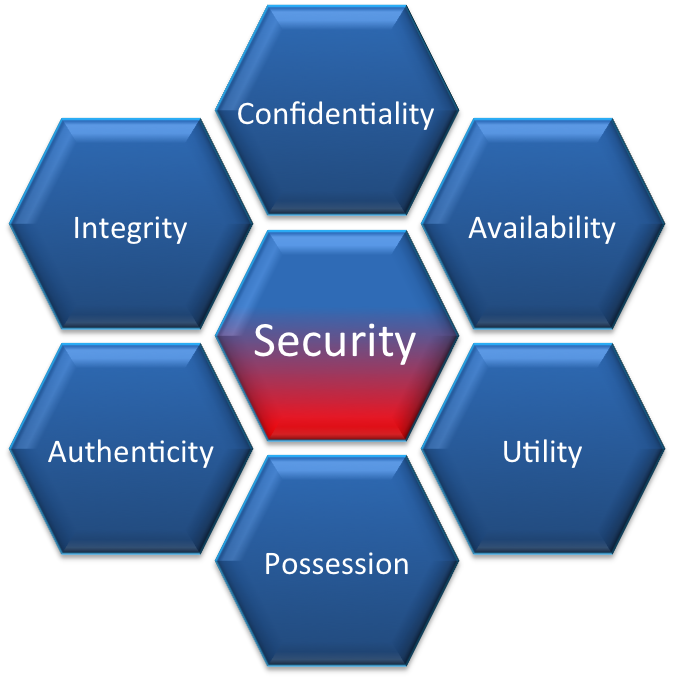
\includegraphics[scale=0.5, natwidth=674,natheight=679]{imgs/hexad.png}
  \caption{Parkerian hexad}
}
\end{figure}
\subsection{Confidentiality}
Tale concetto porta con sé una serie di problemi e di preoccupazioni relative alla trasmissione e alla memorizzazione di dati ricavati dalle operazioni della Smart Grid. Questo tipo di dati, infatti, è spesso ritenuto \textit{confidenziale}, nel senso che se fosse noto, avrebbe tutto il potenziale per causare danni alla sicurezza delle operazioni di tutto il sistema. \newline La confidenzialità, inoltre, può essere intesa anche in un'altra accezione: se i dati fossero noti alla concorrenza, per esempio,  quest'ultima potrebbe trarre un notevole vantaggio in uno specifico settore o in tutto il mercato. \newline A tali fattori si aggiungono altre nuove problematiche legate alla \textit{privacy del consumatore} e, quindi, dei suoi dati, che vengono fuori da meccanismi di metering quali l'AMI. Gli utenti, infatti, si aspettano che i consumi relativi alle loro abitazioni private rimangano confidenziali; se così non fosse, la disponibilità di tali informazioni insieme alla capacità di fare data mining, avrebbe il potenziale per creare significative preoccupazioni sulla privacy. \newline I punti della Smart Grid che introducono rischi per la confidenzialità, sono costituiti da tutte le locazioni in cui sono memorizzati i dati e da tutti i meccanismi di trasmissione delle informazioni. Per quanto riguarda i dati memorizzati, questi potrebbero essere letti, copiati e distribuiti a soggetti diversi dai destinatari. Per quanto riguarda la trasmissione, invece, sia su reti private che su reti pubbliche come Internet, i dati potrebbero essere intercettati, copiati e distribuiti. \newline La soluzione a tali problemi risiede nelle funzioni di \textit{cifratura dei dati} e di \textit{controllo degli accessi}. Fornendo l'appropriato livello di cifratura delle informazioni, quest'ultime possono essere protette da chiunque non sia il diretto destinatario. \newline Il controllo degli accessi, prevede che i dati siano protetti da coloro che hanno l'autorizzazione per accedere al sistema ma che, allo stesso tempo, non hanno bisogno di tali dati per svolgere il loro lavoro.

\subsection{Integrity}
L'integrity si riferisce all'abilità del sistema di evitare che le informazioni possano essere modificate da persone o da sistemi non autorizzati. \newline Se si rendono possibili meccanismi di modifica volontari quali la manipolazione dei dati, o anche involontari quali la loro corruzione, i sistemi riceveranno informazioni non accurate; a lungo andare ciò potrebbe avere un impatto negativo su tutte le operazioni e, in casi estremi, portare ad instabilità o compromettere del tutto la Smart Grid. \newline
I punti della nuova rete elettrica che introducono rischi per l'integrità, sono tutti quei punti che consentono il passaggio dei dati da un sistema ad un altro. Pertanto, la sicurezza di tali meccanismi di transizione è importante, ma ancora più importante è come il sistema che riceve i dati possa assicurarsi della validità di quest'ultimi: se i dati subiscono manipolazioni mentre sono in viaggio tra i due sistemi, il ricevente potrebbe prendere decisioni basate su tali informazioni (che risultano essere errate); se, invece, i dati sono soggetti a corruzione durante la loro transizione, ci si potrebbe trovare di fronte ad un comportamento inaspettato del ricevente. In entrambi i casi, è evidente che l'integrità dei dati sia cruciale per assicurare la stabilità delle operazioni.   \newline
Le risposte ai problemi di integrità, possono essere trovate nei meccanismi di \textit{auditing}, di \textit{authorization}, di \textit{nonrepudiation}, e di \textit{message-signing}, che saranno trattati in seguito (vedi paragrafo 3.3, building blocks).


\subsection{Availability}
Molto spesso si tende ad utilizzare i concetti di reliability ed availability in maniera intercambiabile; in realtà, tali concetti hanno due significati diversi. La reliability, infatti, risponde alle seguenti domande: ``quanto spesso fallisce il sistema?", ``quanto è elastico?"; l'availability, invece, indica la disponibilità del sistema e, quindi, la capacità di compiere il lavoro che gli è stato assegnato, \textit{nel momento in cui se ne ha bisogno}. \newline Una porzione del sistema potrebbe essere attiva, eseguendo e processando i comandi, il 100\% del tempo, e pertanto molto affidabile ma, se le performance non sono adeguate ai bisogni della rete e operazioni critiche vengono ritardate o mancano, non si può dire che il sistema sia disponibile. \newline
I punti della Smart Grid che introducono rischi per la disponibilità sono troppi per poterli elencare: qualsiasi sistema, rete, dispositivo che gestisce le comunicazioni, processo per la gestione dei messaggi, e qualsiasi servizio invocato a qualsiasi livello applicativo e il suo sistema operativo sottostante sono un rischio per la disponibilità quando si trovano a dover gestire l'inoltro di un comando da un'estremità del sistema ad un'altra. Risolvere tale rischio è quasi tanto complicato quanto identificare le componenti del sistema che hanno il potenziale per impattare sulla disponibilità. La maggior parte delle soluzioni si affida a tecniche di ridondanza (clustering, bilanciamento del carico); il costo di tali metodologie, però, cresce in maniera proporzionale ai punti di fallimento che si identificano nel sistema. 

\subsection{Control}
La capacità di controllare le informazioni che necessitano protezione è essenziale per assicurare la loro integrità e la loro usabilità a lungo termine. Ciò ha diverse implicazioni per tutti quei sistemi che si affidano al meccanismo di controllo per scopi di vario genere (legali, normativi o commerciali): se le informazioni utilizzate per calcoli finanziari, come ad esempio i dati ricavati da meccanismi di metering, non fossero controllate, potrebbero compromettere tutti i sistemi che le forniscono e le trasmettono; di conseguenza, la provenienza di tali informazioni non potrebbe essere più garantita, portando una diminuzione dell'affidabilità di quest'ultime. 

\subsection{Authenticity}
Tale termine è spesso utilizzato per descrivere la certezza della provenienza. Il processo di verifica dell'autenticità è simile al processo utilizzato per verificare l'integrità: assicurarsi che la fonte dei dati e i dati stessi, siano autentici.

\subsection{Usability}
Questo aspetto del Parkerian hexad si preoccupa di assicurare che i dati siano utilizzabili. \newline Consideriamo un flusso di dati opportunamente cifrato: quest'ultimo garantisce la sicurezza delle informazioni, ma rende molto difficile far si che queste ultime siano utili. L'usabilità è il fattore che, in definitiva, fornisce valore a livello aziendale e pertanto deve essere preservato e trattato come il requisito con più alta priorità. 

\subsection{Analisi dei rischi}
Quale sarebbe il rischio per l'intero sistema Smart Grid se il sistema stesso, o qualsiasi sua componente, fosse compromessa? Tale rischio e il suo potenziale costo, guidano il lato economico delle decisioni per la progettazione dei meccanismi di sicurezza. \newline Come determinare l'accettazione dei rischi è, pertanto, una decisione legata al business e non una decisione tecnica. Un'azienda che sceglie di adottare una particolare metodologia per l'analisi dei rischi, avrà come input le proprie variabili che guidano le decisioni; tali variabili sono solitamente legate ad un rischio finanziario che l'azienda assume basandosi su una propria analisi competitiva del mercato o su condizioni regolamentari sotto le quali opera. \newline Ci sono altre motivazioni, oltre a quelle finanziarie, che possono guidare l'accettazione dei rischi, come ad esempio fattori legislativi o legati a normative industriali: tali fattori possono portare ad adottare comportamenti che garantiscono la sicurezza anche in assenza di forti incentivi economici, per aggiungere ulteriori capacità di protezione del sistema. \newline È importante riconoscere che nessuna decisione riguardante la sicurezza dovrebbe essere presa senza prima aver considerato i rischi: ``dove sono i rischi nel sistema?", ``Quanto costerà un fallimento del sistema?", ``Quanto costerà un fallimento della sicurezza del sistema?". Un'azienda dovrebbe essere in grado di capire i rischi e dovrebbe essere capace di fare scelte informate ed intelligenti su come risolvere tali problemi. 


\section{Building blocks}
Nel paragrafo precedente, sono state descritte una serie di potenziali minacce e funzioni di sicurezza che sono importanti per sistemi complessi ed interdipendenti come le Smart Grid. \newline In questo paragrafo, si esaminerà una possibile architettura di sicurezza che comprende tutte le funzioni precedentemente analizzate e che cerca di creare una struttura adatta a risolvere tutte le vulnerabilità descritte nel paragrafo 3.2.

\subsection{Layered Security Model}
Il concetto di modello di sicurezza \textit{stratificato} non è un concetto nuovo: i sistemi operativi ed i microprocessori, infatti, lo utilizzano da tempo per controllare gli accessi a  risorse privilegiate. \newline Immaginare tale concetto applicato ad una Smart Grid non è difficile. \newline Dalla figura 3.2 è possibile vedere che la struttura di tale modello è una struttura ad anello in cui la comunicazione tra gli strati del sistema è sicura. In generale, uno strato esterno non può avere libero accesso alle risorse presenti su uno strato più interno; inoltre, le richieste per le risorse non dovrebbero essere in grado di ``saltare" i vari anelli: una richiesta che parte dal terzo anello, non dovrebbe poter accedere direttamente alla risorsa del primo, ma gli accessi sono regolati da opportune interfacce progettate in modo tale da assicurare la sicurezza di tutto il sistema.

\begin{figure}[h]\centering{
  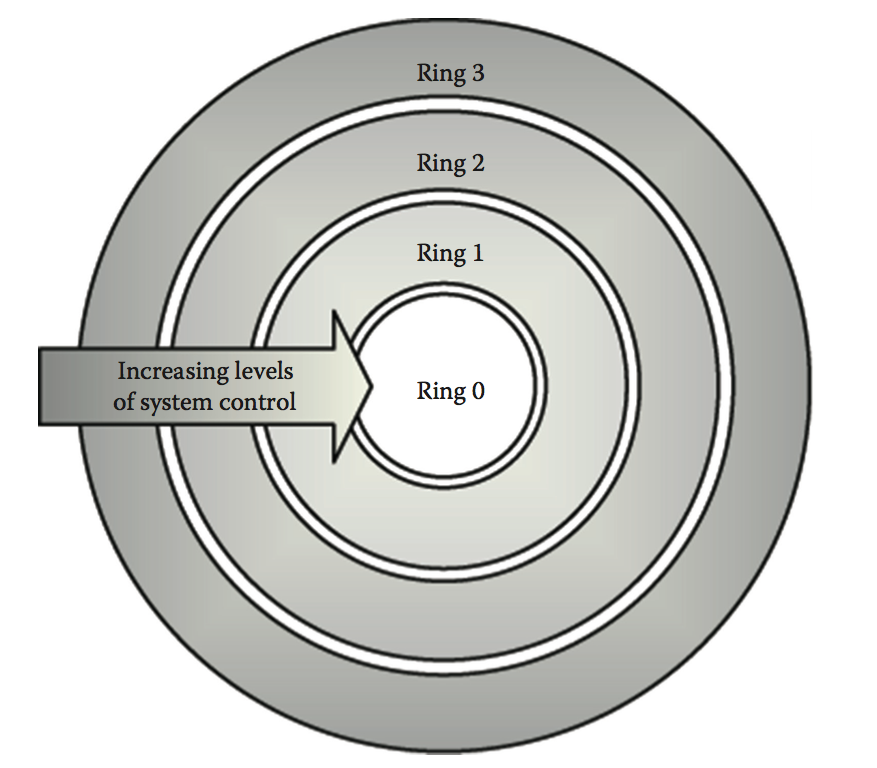
\includegraphics[scale=0.25, natwidth=877,natheight=768]{imgs/ring.png}
  \caption{Layered security model}
}
\end{figure}

Una Smart Grid ben progettata, dovrebbe essere in grado di offrire una simile protezione: i sistemi e le risorse poste agli estremi, come ad esempio dispositivi HAN (home area network) o smart meter, non dovrebbero avere la possibilità di accedere direttamente agli strati operativi (ring 0) della Smart Grid e, in più, i dati che passano per il sistema dovrebbero attraversare opportune interfacce che ne assicurino l'integrità prima di procedere verso strati più interni. \newline
Indipendentemente dal meccanismo specifico utilizzato per separare gli strati, ci sono diversi principi architetturali chiave che dovrebbero essere considerati nel percorso dei dati tra gli anelli: il primo e il più importante è assicurarsi che un fallimento in uno strato non abbia impatto né in uno strato più basso né in qualsiasi sistema dello stesso strato. Con il termine ``impatto" ci si riferisce al fatto che nessuna tra confidentiality, integrity, o availability degli strati sottostanti debba essere colpita. È importante notare, però, che il viceversa non è vero: molto spesso danni ai livelli più bassi si propagano verso gli strati superiori e ciò è dovuto alla natura gerarchica del sistema.
\newline \newline 
Nelle prossime sezioni si analizzano le principali funzioni che costituiscono le componenti di sicurezza di alto livello che la Smart Grid dovrebbe avere per assicurare la protezione del sistema.

\subsection{Authentication}
L'autenticazione è il processo di verifica dell'identità di una persona o di un servizio che richiede l'accesso ad un'altra risorsa. \newline Un meccanismo di autenticazione robusto potrebbe richiedere un certo numero di componenti, ognuna delle quali offre una particolare funzione di tutto il processo. \newline Spesso si tende a pensare all'autenticazione in termini di username e password, il che è corretto, ma non è solo questo: vi può essere autenticazione anche tra sistemi, processi o componenti hardware. Ci sono due componenti base per un meccanismo di autenticazione:
\begin{itemize}
\item \textit{Identity Database}, contiene le informazioni necessarie per determinare chi e cosa sta tentando di accedere al sistema
\item \textit{Identity Management System}, repository centrale di tutte le risorse che richiedono servizi di autenticazione.
\end{itemize}

\subsection{Authorization}
L'autorizzazione è il processo che verifica ciò che la persona o il servizio autenticato può fare all'interno del contesto del sistema. \newline 
Spesso i sistemi più semplici prevedono solo due modalità: ``read-write" e ``write-only"; i sistemi più complessi, invece, dovrebbero fornire regole di autorizzazione più specifiche, includendo la possibilità di indicare quali campi si possono modificare e quali no, solo ad un certo orario del giorno e solamente se autenticati su specifiche macchine.

\subsection{Auditing}
Il cuore di una qualsiasi analisi dei rischi è costituito dal programma di controllo. Senza revisioni periodiche dell'efficacia dei meccanismi di sicurezza che sono in atto nella Smart Grid, non ci sarebbe nessuna garanzia che il sistema sia sicuro. \newline
Un buon programma di controllo dovrebbe essere eseguito periodicamente e dovrebbe testare quelle componenti che sono ritenute essenziali dall'azienda per mettere in sicurezza le operazioni del sistema. Tra i meccanismi più utili per eseguire tali revisioni, vi sono i seguenti:
\begin{itemize}
\item \textit{Logging}: utilizzare file di log e memorizzare al loro interno tutti gli accessi critici al sistema e tutti i cambiamenti avvenuti
\item \textit{Time Synchronization}: in un sistema unificato come una Smart Grid, è essenziale che tutti i dispositivi condividano lo stesso tempo.
\end{itemize}

\subsection{Key Management}
È il processo che gestisce le emissioni delle chiavi per utenti, applicazioni e dispositivi. Tali chiavi sono utilizzate per stabilire l'identità e per assicurare l'integrità dei messaggi quando si inviano comandi tra sistemi. \newline 
Se consideriamo centinaia di chiavi, la loro gestione è relativamente semplice; ma quando ci si trova di fronte a centinaia di migliaia, o addirittura milioni, di dispositivi, la gestione diventa più complessa. Ogni chiave nel sistema sia relativa ad applicazioni, al sistema, ad un dispositivo o ad una persona, dovrebbe poter essere modificata o revocata su richiesta. 
\newline Per fare ciò, si utilizza la ben nota \textit{Public Key Infrastructure} (PKI) [ref.].

\subsection{Message Integrity}
Per trattare l'integrità dei messaggi, consideriamo tre meccanismi: signing, nonrepudiation ed encryption. \newline
Per quanto riguarda il meccanismo di \textit{signing}, quando un messaggio viene inviato da un sistema ad un altro, vi è prima un processo di autenticazione per dimostrare un'identità, seguito da un processo di autorizzazione, per verificare ciò che l'identità può fare. Una volta effettuati questi due controlli, può iniziare lo scambio di messaggi tra i due sistemi. Ci sono due motivazioni principali per cui conviene firmare un messaggio: la prima è assicurare che il contenuto del messaggio non sia stato modificato durante la trasmissione tra i sistemi; la seconda è permettere di verificare l'identità del mittente indipendentemente dal processo di autenticazione. \newline
La \textit{nonrepudiation} entra in gioco quando il mittente di un messaggio necessita di essere riconosciuto (o confermato). Tale termine, infatti, si riferisce alla capacità di fornire una prova inconfutabile, ad una terza parte, di chi ha iniziato una certa azione nel sistema, anche se la persona in questione non sta partecipando al momento. \newline
Il termine \textit{encryption} porta con sé una serie di problematiche e di discussioni ampiamente trattate in letteratura, pertanto è impossibile riassumerlo in poche righe. Si può, però, riassumere il suo scopo: assicurarsi che un messaggio non possa essere letto da una persona o da un sistema che non sono i diretti destinatari dell'informazione. Ciò può essere messo in pratica attraverso innumerevoli algoritmi di cifratura, i quali fanno affidamento sul preservare l'integrità della chiave utilizzata per cifrare i dati; pertanto se tale chiave viene compromessa, lo sarà anche il messaggio. 

\subsection{Network Integrity}
Vi è un'infinità di modi per garantire l'integrità di rete, ognuno dei quali dipende dai dispositivi che la compongono e dalle loro necessità. Infatti, poiché ogni rete ha bisogni diversi, non vi è una configurazione che sia adatta a tutte quante.
\newline Due dei meccanismi principali sono i seguenti:
\begin{itemize}
\item \textit{Firewall}, utilizzato per restringere il traffico sulla rete ad uno specifico insieme di regole. Per esempio, potrebbe limitare il traffico a specifici canali di comunicazione tra un dispositivo e un insieme noto di altri dispositivi.
\item \textit{Rilevamento e prevenzione delle intrusioni}, messo in atto analizzando il traffico della rete per identificare specifici pattern di dati che corrispondono ad attacchi noti.
\end{itemize}

\subsection{System Integrity}
\begin{itemize}
\item \textit{Protezione da malware}, o più comunemente nota come protezione antivirus: ogni sistema dovrebbe avere una strategia che lo protegga da questo tipo di minacce; una protezione robusta, infatti, non solo può evitare che file maliziosi vengano memorizzati, ma può anche far si che si possa avvisare un operatore del ritrovamento del malware. 
\item \textit{Gestione della configurazione del sistema}: le specifiche su come un sistema è configurato possono impattare enormemente sulla sua sicurezza. La gestione è necessaria per assicurarsi che il sistema non cambi rispetto alle basi di funzionamento stabilite.
\item \textit{Validazione e testing}: essenziali per garantire l'integrità del sistema. Prima di effettuare qualsiasi cambiamento e di distribuire nuovi sistemi, bisogna valutare le nuove modifiche e capire che impatto hanno sull'intero sistema. I cambiamenti devono essere testati per sicurezza e per garantire che non abbiano conseguenze negative sull'affidabilità di tutto il sistema.
\end{itemize}

\section{Minacce e loro impatto}

\section{Sforzo dello stato (?)}

\section{Compagnie}

\section{Servizi di terze parti}

